

\beginsong {Studentsång}[ 
by = {Herman Sätherberg},
index = {Sjungom studentens lyckliga dag}]

\beginverse* 
Sjungom studentens lyckliga dag,
låtom oss fröjdas i ungdomens vår!
Än klappar hjärtat med friska slag,
och den ljusnande framtid är vår.
/: Inga stormar än 
i våra sinnen bo.
Hoppet är vår vän 
och vi dess löften tro,
när vi knyta förbund i den lund,
där de härliga lagrarna gro
där de härliga lagrarna gro.
Hurra!:/
Hurra!
\endverse
\endsong
\begin{intersong}
	\begin{center}
		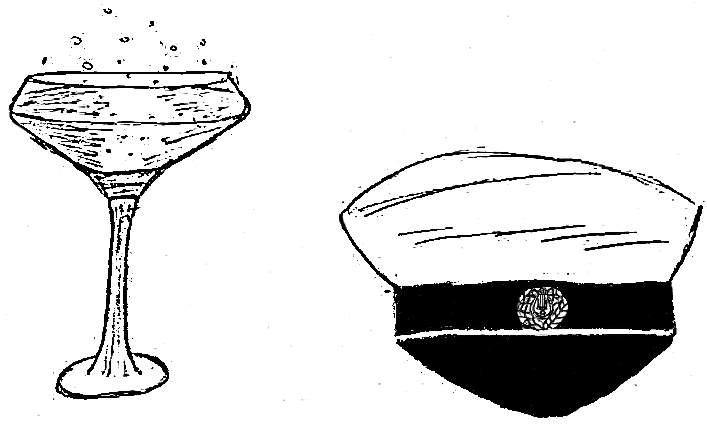
\includegraphics[width=1\textwidth]{../bilder/fardigabilder/CamillasFardigaBilder/Studentsangen2.png} 
	\end{center}
\end{intersong}